\documentclass[11pt, letterpaper]{article}

\usepackage[english]{babel}
\usepackage[utf8x]{inputenc}
\usepackage[gen]{eurosym}
\usepackage{amsmath}
\usepackage{amssymb}
\usepackage[dvipsnames]{xcolor}
\usepackage{graphicx}
\usepackage[stable]{footmisc}
\usepackage{caption}
\usepackage{subcaption} 
\usepackage[title]{appendix}

\captionsetup{font=footnotesize}


 
\title{Project report: Equilibrium in Energy Markets}
\author{P\'ia Amigo, Sebasti\'an Cea, Felipe Feijoo}
\date{June 17, 2019}

\begin{document}
\maketitle

\begin{abstract}
In this report we present the current status of the project: Equilibrium in Energy Markets. Our project consists in the study of the chilean energy markets in the context of a cap-and-trade scheme.  We provide a basic introductions of microeconomics and the formulation of Mixed Complementarity Problems to solve equilibrium analysis. We describe the work of de Maere et. al. 2018, which is the motivation of our project. Lastly, we introduce our project by discussing the cap-and-trade policy, and formulating a first approach to the model, based in the theoretical framework provided in de Maere's work. 
\end{abstract}

%\section{Draft}
%\color{Red}
%Proposed topics for the report:
%\begin{itemize}
%\item Complementarity modelling in Energy Markets
%    \begin{itemize}
%        \item Supply and Demand
%        \item Market Equilibrium
%        \item Social Welfare
%        \item Formulation of Mixed Complementarity Problems (MCP)
%    \end{itemize}
%\item The paper: Risk trading in capacity equilibrium models
%\begin{itemize}
%    \item Incomplete markets
%\end{itemize}
%\item Future prospects: Applications
%
%\end{itemize}

\color{Black}

\section{Some Basic Concepts in Microeconomics}

Microeconomics is a social science that studies the decisions of individuals and firms to allocate resources of production, exchange, and consumption. It also deals with prices and productions in single markets, and the interaction between different markets. 

In this section, we will review some basic concepts in Microeconomics, that are relevant for the development of our project. Particularly, we will discuss the classic topic of Supply and Demand, Social Welfare, Equilibrium, Competition, among others. 

\subsection{Supply and Demand}
The supply and demand model is useful to explain how price and quantity
traded are determined and how external influences affect the values of those variables. A simple definition of each is the following:
\begin{itemize}
    \item[] \textbf{Supply} is the willingness of \textit{producers} to offer a given quantity of a good or service for a given price. 
    \item[] \textbf{Demand} is the willingness and ability of \textit{consumers} to purchase a given amount of a good or service at a given price.
\end{itemize}


For the sake of simplicity, we will describe the supply and demand  model for a single-commodity market. The firms in the market will not try to change the price of the commodity, i.e., they are \textit{price-takers}.

\smallskip

The law of demand is based on the \textit{universal} observation that as the price of a good rises, consumers will choose to buy less of it, and as its price falls, they buy more\footnote{This observation is valid for any type of good, although there are rare exceptions.}. The price, is then, important in the decision of the consumer, but it is not the only variable that influences the decision; other variables might be  consumers' incomes, their tastes and preferences, the prices of other goods that serve as substitutes or complements, etc. (for our purposes, we will only deal with price).  
This behaviour is represented through the demand function, which gives the total demand quantity $q$ of a certain good
\begin{equation}
    q_d=f_d(p)
\end{equation}

The other side of the story is the law of supply. In general,
producers are willing to sell their product for a price as long as that price is at least as high as the cost to produce an additional unit of the product. This means that the supply depends on the selling price but also in the cost of production for an additional unit of the good. This cost of productions depends on the technology employed in the production process (e.g. land, labor, capital, and materials). Again, we will define the supply function only depending on the price, for simplicity. 
The supply function, which gives total supplied quantity $q$ is 
\begin{equation}
    q_s=f_s(p)
\end{equation}

Most of the cases, economists are interested in the inverse supply and demand functions, that is, in terms of the price:
\begin{align}
    p= & f^{-1}_d(q) \\
    p= & f^{-1}_s(q)
\end{align}

Figure \ref{demand} shows the relationship between price and quantity for the law of demand, and Figure \ref{supply} shows the law of supply. 

\begin{figure}[ht!]
  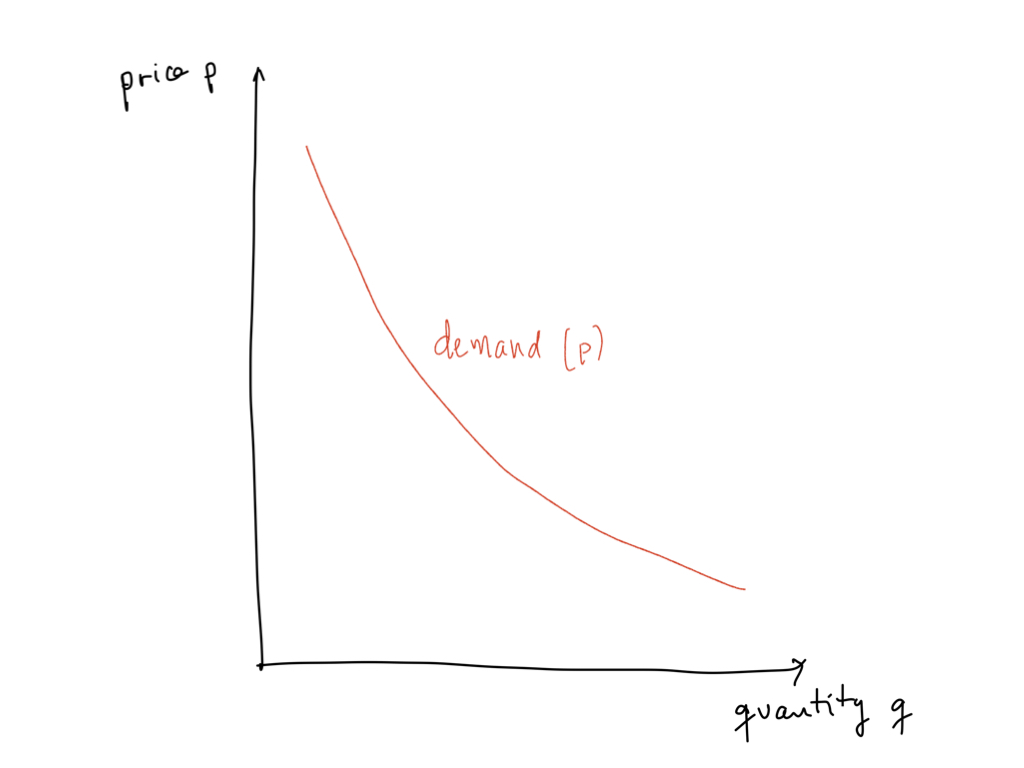
\includegraphics[width=\textwidth]{Informe/demand.jpeg}
 \caption{Law of Demand. The demand curve has a negative slope because a higher selling price tends to induce a smaller quantity demanded.}
 \label{demand}
\end{figure}
 
\begin{figure}[ht!]
  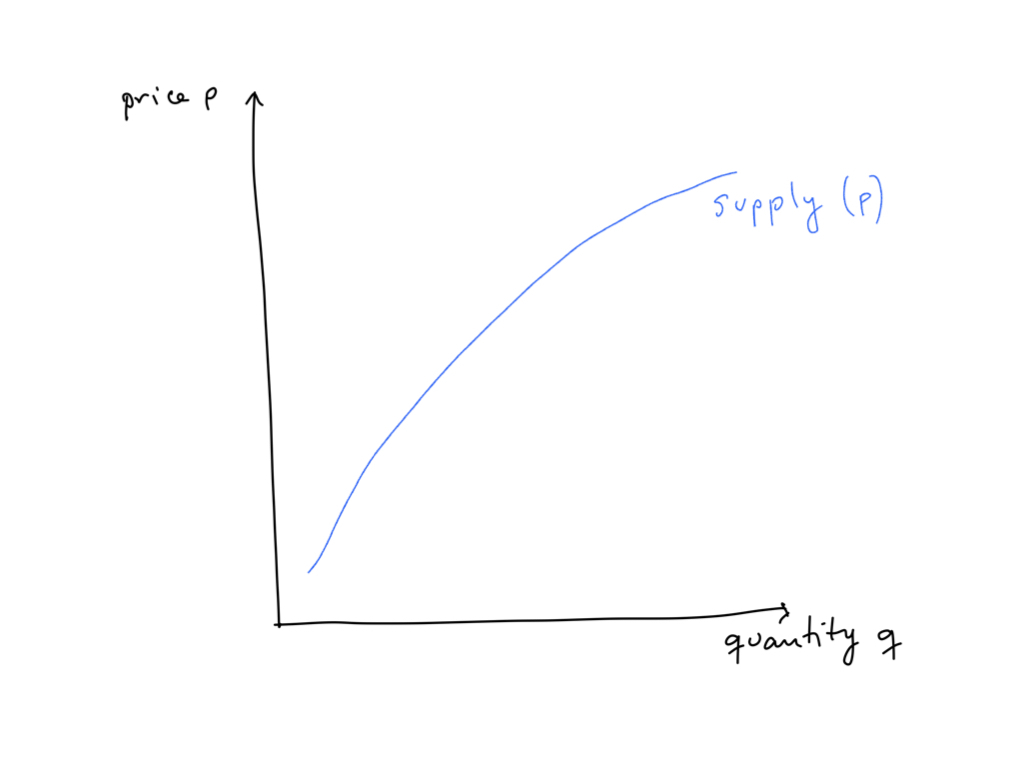
\includegraphics[width=\textwidth]{Informe/supply.jpeg}
 \caption{Law of Supply. The supply curve shows that a higher selling price tends to induce a larger quantity supplied, and thus, the slope is positive.}
 \label{supply}
 \end{figure}

\subsection{Market Equilibrium}

From Figures \ref{demand} and \ref{supply} we can conclude that higher prices cause consumers to buy less and producers to produce more. This means that there can be only one price at which the quantity produced equals the quantity purchased. When that condition is met, we say that the market has reach its \textbf{equilibrium}.  Graphically, it is the intersection at $(q^{\ast},p^{\ast})$ of the demand and supply curves, as shown in Figure \ref{equi}.  We can interpret this equilibrium as the highest price a buyer is willing to pay is just equal to the lowest price a seller is willing to accept for that same quantity.

 \begin{figure}[ht!]
  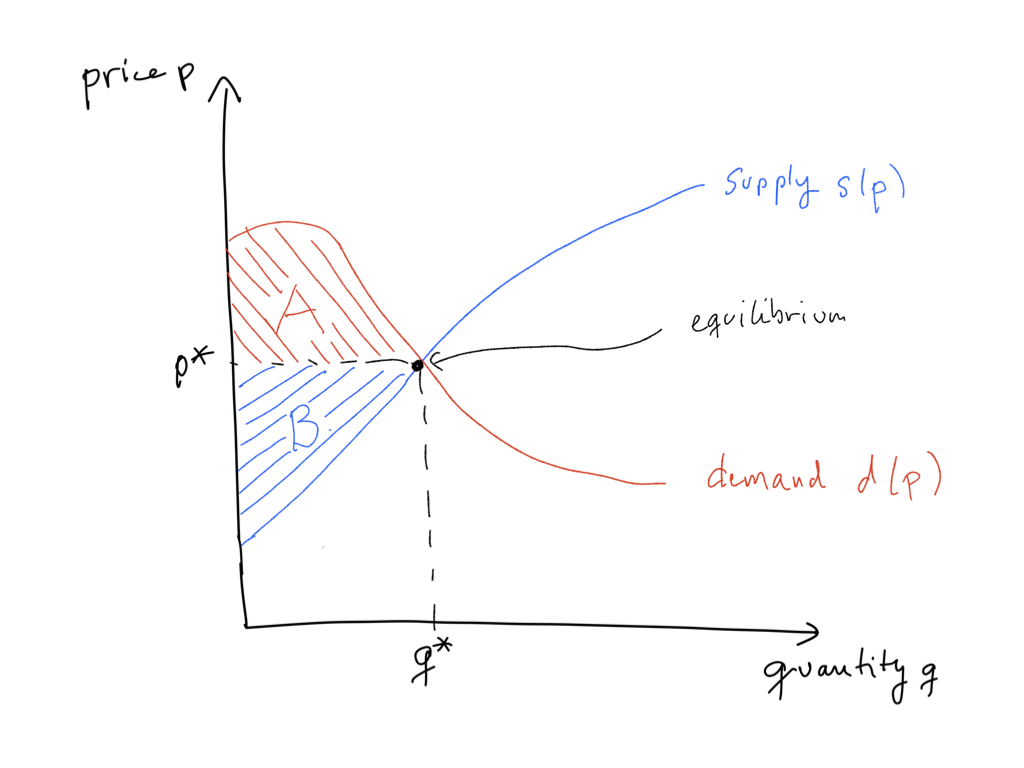
\includegraphics[width=\textwidth]{Informe/equilibrium.jpeg}
 \caption{Equilibrium (q∗, p∗), consumers’ surplus (area A), and producers’ surplus (area B)}
 \label{equi}
\end{figure}

Intuitively, the word equilibrium tells us that any deviations from the price $p^{\ast}$ are naturally corrected, and $q^{\ast}$ is the quantity that corresponds to $p^{\ast}$. Producers will try to produce and sell more than consumers are willing to buy. This will result in an excess of the supplied quantity compared with the demanded quantity, or a \textbf{surplus}. To sell the surplus, producers need to lower the price. As the price decreases, the demand will rise, until they meet at equilibrium. The same happens in the opposite way: if the price is too low, consumers will want more, and the demand increase, until appears a shortage situation, where the high demand cannot be satisfied by producers. But producers react and they increase the price until the demand drops and again, with time, they meet again at equilibrium.

Algebraically, the simplest way to find equilibrium price is by setting the demand function equal to the supply function and solving for price.
Any variables other than price and quantity are determined outside of the demand and supply model of the market, and thus, are called exogenous variables. Price and quantity, however, are determined within the model for this particular market and are called endogenous variables. The equilibrium is then solved as a system of equations, to solve it we need another equation: the equilibrium condition
\begin{equation}
    q_d=q_s
\end{equation}
This equation simply says that all the demand must be satisfied by the supply.
\smallskip
 
The value of the exogeneous variables of our system of equations can be considered as \textit{given}, but in fact, those values are determined in other markets, such as markets of labor or other goods. When we take into account all the feedback mechanisms between several markets simultaneosuly, we are performing a \textbf{general equilibrium analysis}. Instead, we can gain enough information from real historical data that describes the market, and thus use this given values of exogenous variables to solve a \textbf{partial equilibrium analysis}.

\subsection{Social Welfare Optimization}

The \textbf{social welfare}  (SW) is the result of adding the consumer and the producer surplus and it represents the net gain of all participants in the market, due to selling or buying. It is possible to calculate the SW at any value of quantity, and we can define the $SW$ function as
\begin{equation}
    SW(q)=\int_0^q f^{-1}_d(q')dq' - \int_0^q f^{-1}_s(q')dq'
\end{equation}

An alternative way to find the equilibrium is to find the value $q$ that maximizes the $SW$ function (Gabriel et. al. 2013):

\begin{align}
    \textrm{Maximize} & \quad SW(q)\\
    \textrm{which implies that} & \quad \frac{dSW}{dq}=0\\
    \textrm{which implies that} & \quad f^{-1}_d(q)- f^{-1}_s(q)=0\\
    \textrm{Therefore} & \quad f^{-1}_d(q) = f^{-1}_s(q)
\end{align}

In the above equation it has been assumed that that the inverse demand function has a negative slope, and that the inverse supply function has a positive slope so we can conclude that $SW(q)$ is strictly concave. Thus, the maximum point it is unique, and defined by the condition that the derivative is zero.

This relation between equilibrium and SW means that the market tries to maximize a single objective function, that works for all the agents in the market. The important concept behind this is the so-called \textit{Pareto optimality}. An economic situation is said to be Pareto optimal (or Pareto efficient) if it is impossible to make an improvement for any agent without making things worse for another agent\footnote{This is not always the case, and there are several of examples where the market is not Pareto optimal, but the details go beyond the scope of this report.}. 

Let us assume we have a market where firms are price-takers. The variable cost of firm $i$ as a function of $q_i$ is $VC_i(q_i)$. The firm expects to receive a price $p$ for a supply of quantity $q_i$, so the profit of the firm is $pq_i-VC_i(q_i)$, and the maximum of that profit occurs when  $p-\frac{VC_i(q_i)}{dq_i}=0$, provided that $VC_i(q_i)$ is a continuously
differentiable and strictly convex function. To calculate the SW, we can combine all the firms in one equation , and the SW maximization results in
\begin{align}
    \textrm{Maximize} & \quad \int_0^q f^{-1}_d(q')dq' - \sum_i VC_i(q_i)\\
    \textrm{s.t} & \quad q - \sum_i q_i = 0 \quad (\lambda)
\end{align}

The constraint requires that the sum of all firms’ outputs must equal the demand. $\lambda$ is the dual variable of the constraint\footnote{More details on dual variables are given in the next section.}. 
This is a simplistic model, but we can stretch it a bit to add more realism to the model. For instance, a production process defined a combination of  production technology, raw materials, and geographical location-dependent factors such as costs of transportation to the market. So, the cost can have a little more complex format.
If we consider that the production process consists in several steps, $b$ is the index of this steps, and the output at the end of each step is quantity $x_{ib}$. Each process has a maximum capacity $K_{ib}$, and $x_{ib}$ cannot surpass it. Also, $x_{ib}$ is always non-negative. The maximization of $SW$ can be expressed as a minimization problem of the cost (making the appropiate changes to the signs in the expression)
\begin{align}
     \textrm{Maximize} & \quad \sum_i \sum_b c_i x_{ib} - \int_0^q f^{-1}_d(q')dq' \\
    \textrm{s.t} & \quad q - \sum_i \sum_b x_{ib} = 0 \\
                 & \quad x_{ib}-K_{ib} \leq 0 \quad \forall i,b\\
                 & \quad -x_{ib} \leq 0 \quad \forall i,b
\end{align}

The equilibrium problem is then a set of optimization problems for all the firms. We will see in section \ref{MCP} that, using the Karush-Kuhn-Tucker conditions of the optimization problem, we can solve this equilibrium problem as a Mixed Complementarity Problem (MCP). 

\subsection{Nash Equilibrium}


The Nash equilibrium is a concept of game theory that consists in the analysis of the outcome of the strategic interaction of several decision makers. In this interaction, it is not possible to predict the result of the choices of the players individually but instead, one have to take into account the decision of all the players involved in the game. 
Using this idea to market equilibrium, we can consider the agents of the market as the players in the game, indexed by $i$. The strategies each agent chooses are denoted by the vector $x_i$. Each agent is interested in maximizing its utility $U_i$. In the Nash paradigm this utility $U_i$ depends not only on the values of the player’s own variables $x_i$, but also on the values of other players's. We can write this explicitly as $U_i(x_i,x_{-i}$, where $-i$ means all the other agents but itself. Then, the Nash equilibrium is found by solving the set of optimization problems for all players:
\begin{equation}
    \textrm{choose} \quad x_i \quad \textrm{to maximize} \quad U_i(x_i,x_{-i})
\end{equation}

This is the simplest Nash game; complications may arise when there are constraints linking the involved agents. This problem is called a Generalized Nash Equilibrium, but we will not go into details. The interested reader may refer to Chapter 3 in Gabriel et al. (2013). 

\section{Formulation of Mixed Complementarity Problems\footnote{The formulation presented here is taken from the book \textit{Complementarity Modelling in Energy Markets}, (Gabriel et al., 2013) } } \label{MCP}

Complementarity models can represent the simultaneous optimization
problems of one or several interacting decision-makers, and thus they have become an increasingly important and powerful tool for formulating and solving bottom-up energy market models (Ruiz et al., 2014). These models focus on the outcomes of the actions of economic agents, where economic agents can either be individuals (as producers and consumers) or organizations that deliver goods or services (Murphy et al., 2016).

In this section we will provide an glimpse of Mixed Complementarity Problems (MCP) and how their formulation is a powerful tool regarding the solution of equilibrium problems. 

\subsection{MCPs and Optimization}

Formally, the Mixed Complementarity Problem (MCP), given a function $F: \mathbb{R} \longrightarrow \mathbb{R} $ is to find vector $x \in \mathbb{R}^{n_1}$ and $y \in \mathbb{R}^{n_2}$ such as, for all $i$:
\begin{itemize}
    \item $F_i(x,y) \geq  0$, $x_i \geq 0$, $x_i \cdot F_i(x) = 0 $, $i=1,..., n_1$
    \item  $F_{j+n_1}(x,y) = 0$, $y_j \ {\textrm free}$, $j=1,...,n_2$
\end{itemize}

Usually, the first conditions are written in the form $ 0 \leq F(x) \perp x \geq 0$, where the $\perp$ operator indicates the complementarity.

In practice, the MCP can be formulated from an optimization problem. We will described in the following paragraphs how we can establish a MCP problem from an optimization program, reviewing the concepts of optimization problem, Lagrangian functions, Karush-Kuhn-Tucker conditions and equilibrium problems.

The general form of an optimization problem (also known as mathematical programming) is as follows:

\begin{align} \label{eq:opt}
         & \min_x f(x)  \\
    \textrm{ s.t} \ \ \  & h(x) = 0 \\
        \ \ \  & g(x) \leq 0
\end{align}

where $f: \mathbb{R}_n \longrightarrow \mathbb{R}$ is the objective function, $x \in \mathbb{R}_n$ is the optimization variable vector, and $h(x)$ and $g(x)$ are the equality and  inequality constraints, respectively. The set of solutions meeting the constraints $h(x) = 0$ and $g(x) \leq 0$ constitutes the feasible region, and the feasible solution that minimizes the function $f(x)$ is the optimal solution $x^{*}$. The function $f(x)$ at point $x^{*}$ is the objective function optimal value.

For the optimization problem established above, we can define the Lagrangian function $\mathcal{L}$:
\begin{equation}
     \mathcal{L} = f(x) + \lambda^{T} h(x) + \mu^{T} g(x)
\end{equation}


where $\lambda$ and $\mu$ are the Lagrange multipliers associated with the equality and inequality conditions, and $f(x)$, $h(x)$ and $g(x)$ are continuosly differentiable functions in the feasible region. The use of the Lagrangian multipliers is a useful method to solve optimization problems. The main idea is to find the points where the functions $f$, $g$ and $h$ are tangent to each other (the optimal points). This is the same as finding the points where the gradient vectors of $f$, $g$ and $h$ are parallel to each other. This can be achieved by finding the gradient of the Lagrangian function and setting it to zero, i.e.,
\begin{equation} 
     \nabla \mathcal{L} = 0
\end{equation}



In this context, we can interpret the value of the Lagrangian multipliers as the rate of change of the solution to the constrained optimization problem as the constraint varies. This is also known as the shadow price: it tells you how much more profit you would get by increasing the amount of a resource by one unit.

As established at the beginning of this section, we will use MCP formulation - and not the Lagragian multipliers - in our problems, but this description of the Lagragian function and its gradient is useful to enunciate the Karush-Kuhn-Tucker (KKT) conditions, essential to the MCP formulation method.

The KKT are necessary (but not sufficient) conditions for a solution to be optimal. The formulation of the KKT conditions is obtained as follows:

\begin{align}
    \textrm{Stationarity}: \ \  &  \nabla_x f(x) + \lambda^{T}  \nabla_x h(x) + \mu^{T} \nabla_x g(x) \\
    \textrm{Primal Feasiblity}: \ \  &  h(x)=0 \ \textrm{and} \ g(x) \leq 0  \\
    \textrm{Dual Feasibility}: \ \  & \mu \geq 0 \\
    \textrm{Complementary Slackness}: \ \  & \mu^{T} g(x) = 0 
\end{align}

A solution $x$ of an optimization problem, with $f(x)$ is a continously differentiable convex function and $h(x)=0$ and $g(x) \leq 0$ constitutes a convex set, and the solution $x$ satisfies the KKT conditions, is guaranteed to be an optimal solution.

The condition that guarantees sufficiency is 
\begin{equation}
    \nabla^{2}_{x} f(x) + \lambda^{T} \nabla^{2}_{x} h(x) + \mu^{T} \nabla^{2}_{x} g(x) \geq 0
\end{equation}

on the subspace
\begin{equation}
    y: \nabla_{x} h(x) y =0; \nabla_{x} g_j(x) y =0, \forall j \in \mathcal{J}\}, \mathcal{J} = j; g_{j}(x) = 0, \mu_{j} > 0
\end{equation}


This subspace is the tangent hyperplane at $x$. In other words, the Hessian of the Lagrangian function at $x$ should be positive definite on the tangent hyperplane at $x$.

\begin{figure}[ht!]
  \begin{center}
    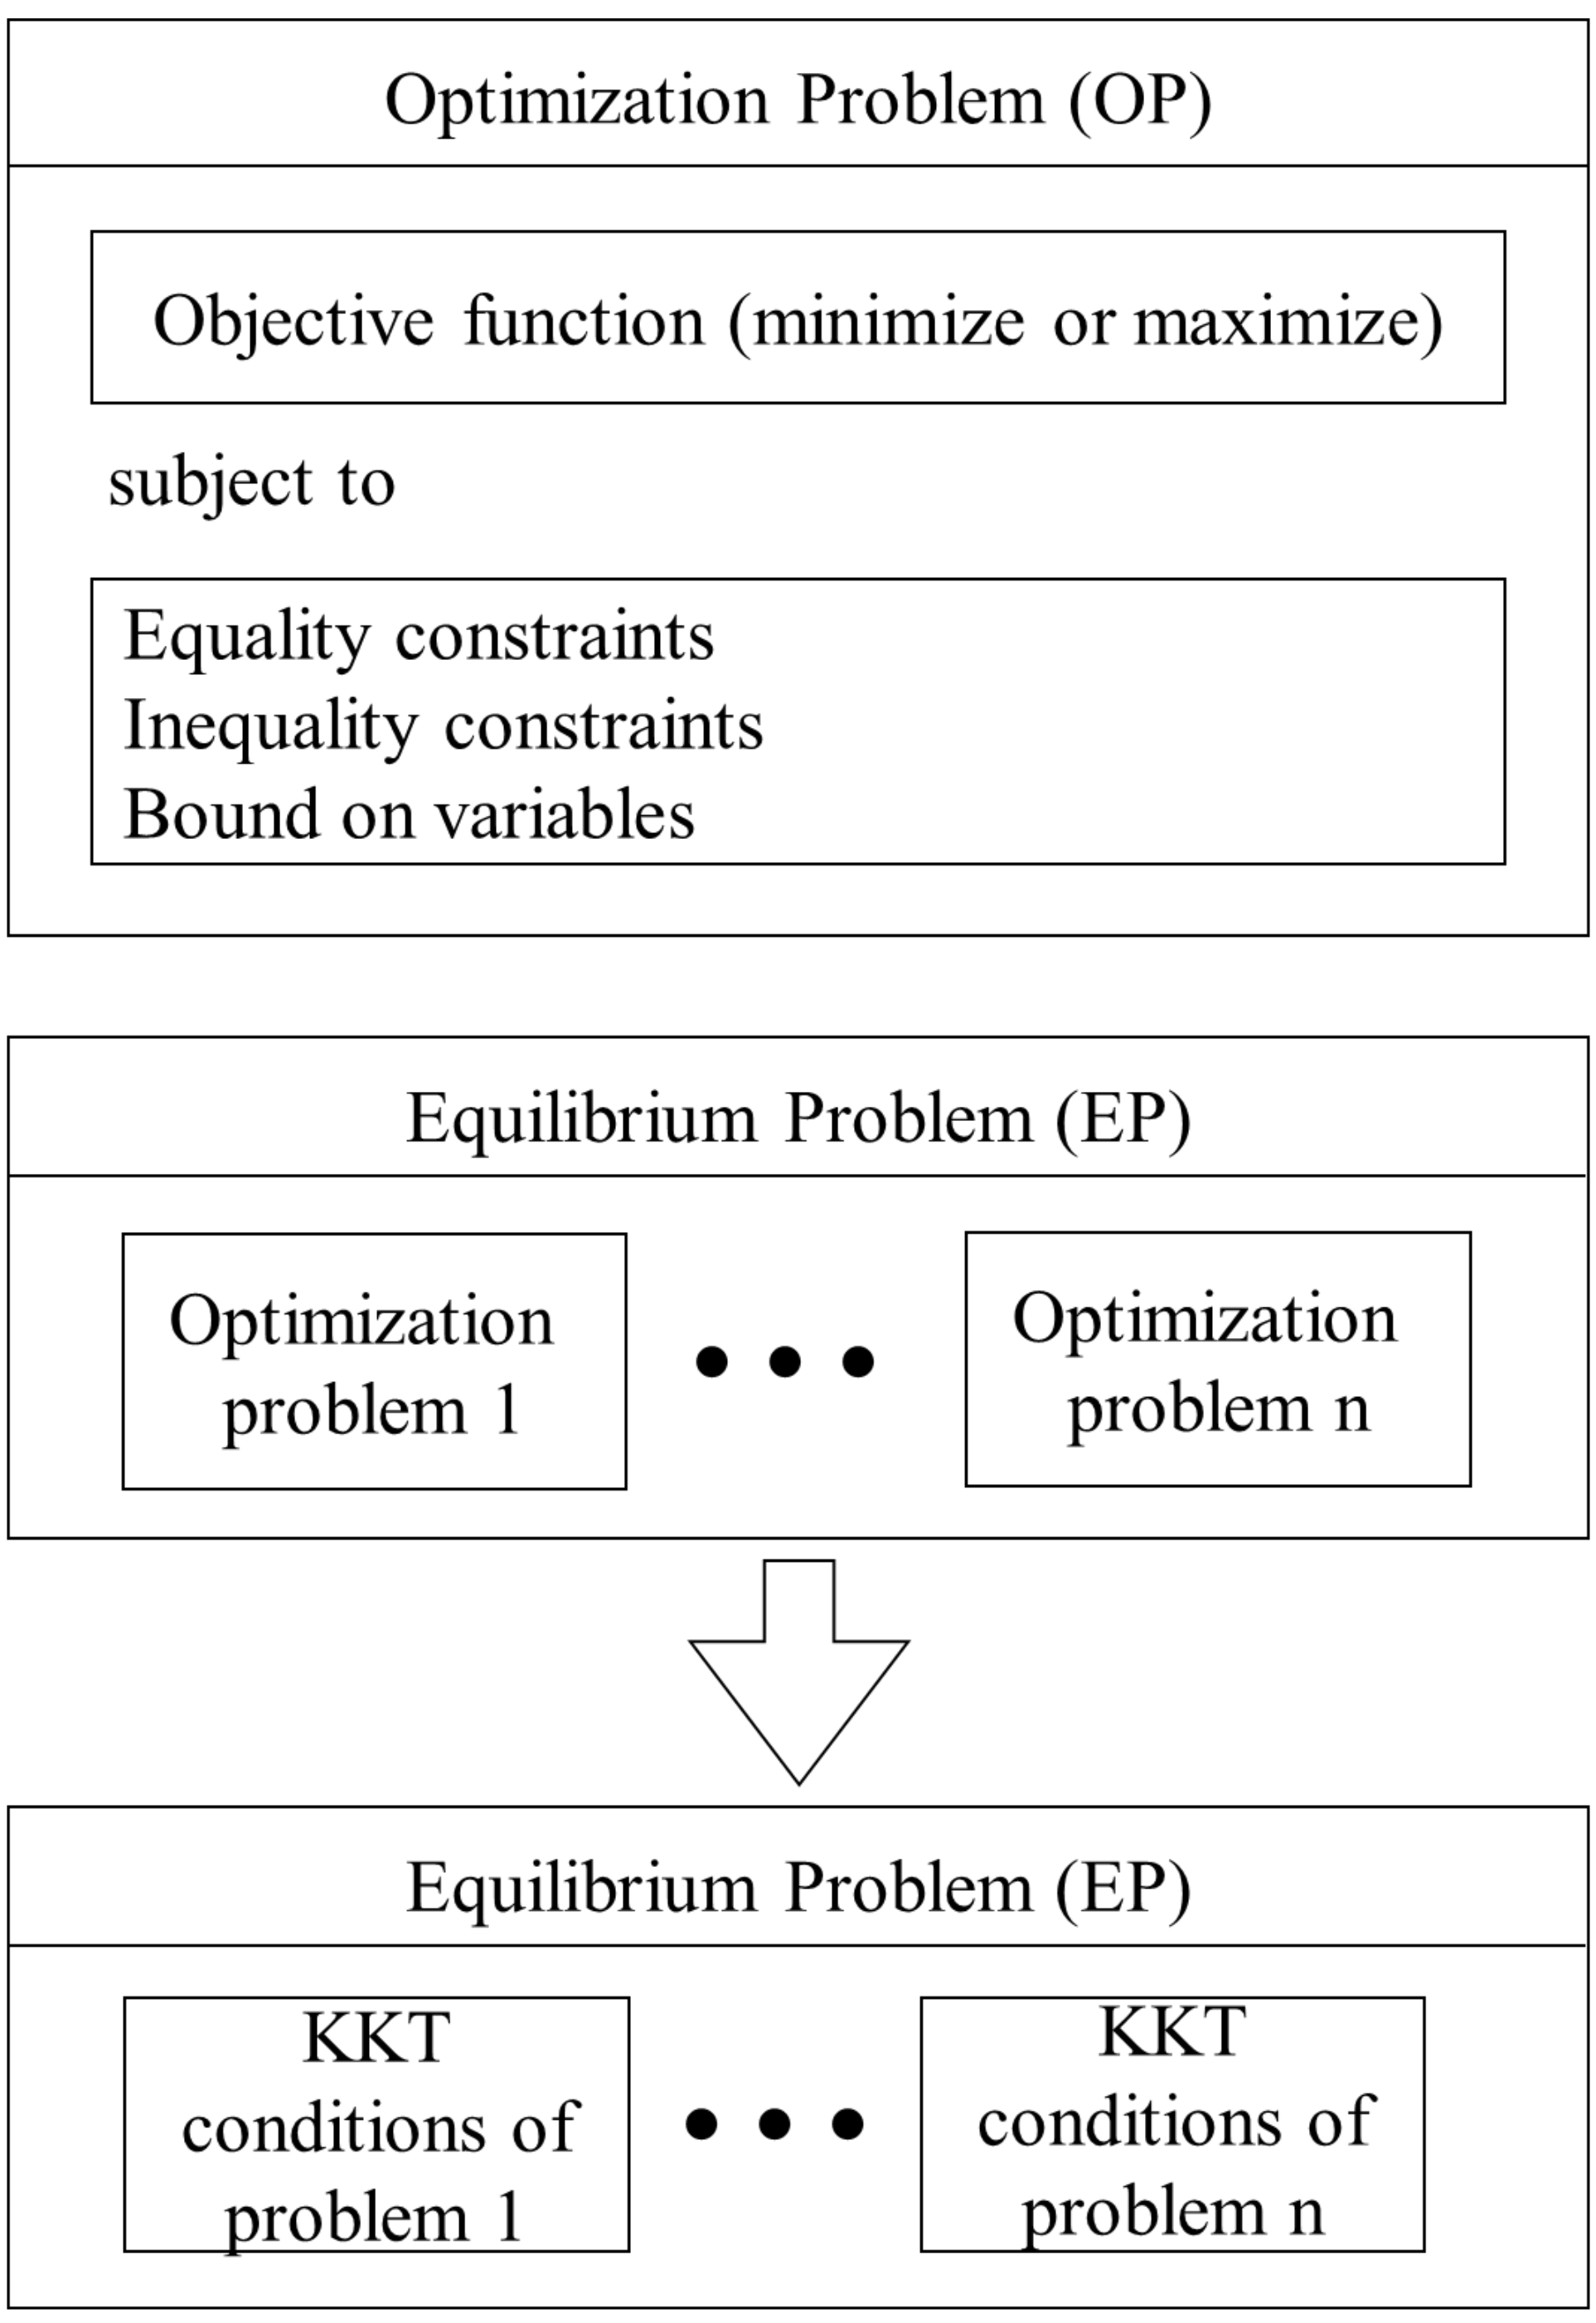
\includegraphics[width=6cm]{Informe/EP.png}
  \end{center}
 \caption{A set of optimization problems that constitutes an equilibrium problem can be formulated as a complementarity problem using the KKT conditions (figure adapted from Gabriel et al., 2013, chapter 2). }
 \label{opt-eq}
\end{figure}

\subsection{Market Equilibrium and KKT Conditions}

For our purposes, we can define equilibrium of a market in a simple way: The collection of all behaviours and strategies of all the agents (i.e. producers and consumers) involved in the market, together with conditions that express the interactions of their decisions and a condition that express the interaction between agents, the market clearing condition (Gabriel et al., 2013). 
\smallskip

Complementarity is a natural way to compute equilibrium problems among market players whose profit maximization problems are stated as optimization problems (Ruiz et al., 2014). One of the advantages is that modern solvers such as PATH, implemented in GAMS (Ferris \& Munson, 2000) can manage a high number of variables, thus the complementarity formulation gives rich details concerning supply options, demand variability and other constraints. 
As shown in Figure \ref{opt-eq}, the simultaneous optimization problem of all the market agents is represented by the KKT conditions of each optimization problem, and the solution is the equilibrium of the problem. 



\section{Capacity Expansion Equilibria}\label{paperI}
Our project's starting point is the paper ``Risk trading in capacity equilibrium models'' (de Maere et al., 2018, working paper\footnote{https://www.eprg.group.cam.ac.uk/eprg-working-paper-1720}, hereafter Paper I). In this paper, the authors present a set of power investment models, that include risk trading and different assumptions on perfect and imperfect markets. The main purpose is to provide a unifying computational framework formulated as stochastic Nash equilibrium models. This type of analysis, stochastic equilibria under risk, is certainly valuable for power generation companies (gencos) to forecast power prices or to put financial value to investment. Policy makers and regulators also can see the outputs of this analysis beneficial to asses economic efficiency (or inefficiency) of existing proposed markets. In section \ref{future}, we will use this framework in a real-world problem of cap-and-trade policy in Chile.

The following sections  will describe the details of the model presented in Paper I.

\subsection{General Overview}
Power capacity expansion is a type of stochastic equilibrium. The model is structured as a noncooperative Nash game of $N$ agents and the analysis is conducted as a two stage problem. The stochasticity is characterized by a number of stochastic scenarios $\omega \in \Omega:=\{1,...,K\}$ and the space of uncertain outcomes (costs) is $\mathcal{Z}:=\mathbb{R}^K$.
\smallskip

Each agent $i$ has associated a strategy set $X_i \subset \mathbb{R}^{n_i}$. The vector of design variables $x_i$ is the agent $i$'s investment (capacity)  in a risky asset $\Xi_i$ (cost from production plant to operate in an uncertain market) is $\Xi_i(x_i,x_{-i}):= (\Xi_{i\omega}(x_i, x_{-i})) \in \mathcal{Z}$. This decision is made in the plant's present -- the first stage of the model. Each scenario cost $\Xi_{i\omega}(x_i, x_{-i})$ is the optimal value of a production optimization problem carried out by agent $i$. At the second stage (the spot market in the uncertain future) the agent $i$ chooses its production quantity $y_i$ given the plant capacity and operating costs determined in the first stage. 
\smallskip

Paper I makes two considerations regarding risk: i) the agents are risk neutral or ii) the agents are risk-averse, and hedge the risk with financial products. We will describe both cases. For the sake of simplicity, the paper considers only two agents -- a genco and a consumer or retailer.

\subsubsection{Risk Neutral Agents}
If the agents are risk neutral, the cost is evaluated as an expected value of any cost $Z \in \mathcal{Z}$, with probability $\Pi \in \mathcal{P}$, i.e.,
\begin{equation}
     \mathbb{E}_{\Pi}[Z]:= \sum_{\omega} \Pi_{\omega}Z_{\omega}
\end{equation}

In many cases, the probability comes from real data (physical probability). 
\smallskip

The two stages of the problem are:

\begin{itemize}
    \item First Stage is capacity investment with convex investment cost $Ix$
    \item Second stage is stochastic spot market in scenario $\omega$, where the producer or genco $G$ wants to optimises production $Y_\omega$ at cost $C_\omega$ and with price $P_\omega$:
    \begin{equation}
         V_{G\omega}(x, P_\omega):= \min_{Y_\omega} C_\omega Y_\omega - P_\omega Y_\omega \ \ \textrm{s.t. \ \ } 0 \leq Y_\omega \leq x
    \end{equation}
    The retailer optimizes consumption $Q_\omega$ given price $P_\omega$ and $U_\omega$ is the utility of consumption:
    \begin{equation}\label{eq:RN_Rspot}
        V_{R \omega} (P_\omega):= \min_{Q_\omega} P_\omega Q_\omega - U_\omega Q_\omega \ \ \textrm{s.t. \ \ } Q_\omega \geq 0 
    \end{equation}
    
    
The price of electricity $P_\omega$ clears the spot market:
    \begin{equation}\label{eq:mccRN}
        0 \leq Y_\omega - Q_\omega \perp P_\omega \geq 0
    \end{equation}
    
\end{itemize}

The equilibrium is established by solving the second stage stochastic program:

\begin{itemize}
    \item[1.] For the Genco
        \begin{align}
             \min_{x,Y} & \quad Ix + \mathbb{E}_{\Theta}[C_\omega Y_\omega - P_\omega Y_\omega] \\
             \textrm{s.t} & \quad  x \in X\\
                          & \quad  0 \leq Y_\omega \leq x  \ \ \forall \omega
            \end{align}
    \item[2.] The Retailer solves equation (\ref{eq:RN_Rspot}) .
    \item[3.] The price clears spot market by equation (\ref{eq:mccRN}) in each scenario $\omega$.


\end{itemize}

\subsubsection{Risk Averse Agents}\label{sec:RN}

A risk-averse agent values the cost in uncertain scenarios through a risk function in the form $r_i(\Xi_i(x_i,x_{-i}))$ with $r_i: \mathcal{Z} \rightarrow \mathbb{R}$. To hedge the risk, the agent also decides to buy financial products $W_i \in \mathcal{W}$, where $\mathcal{W}$ is unconstrained in $\mathcal{Z}$, (i.e., $\mathcal{W}=\mathcal{Z}$ complete market) and the cost is $r_i(\Xi_i(x_i,x_{-i}) - W_i)$. The cost of these financial products or contracts is the price of risk $P^{r}$.  
In this case, for the spot market, the optimization for agent i is 
\begin{equation}
    \min_{x_i, W_i} P^{r} W_i + r_i(\Xi_i(x_i,x_{-i}) - W_i) \ \ \textrm{s.t \ \ \ } x_i \in \mathcal{X}, W_i \in \mathcal{W}
\end{equation}

and the price of risk $P^r$ is determined by the equilibrium condition in the risk trading market :
\begin{equation}
    \sum_i W_i =0
\end{equation}
that is, all the financial products balance each other.

The risk aversion, or the risk function, is modeled as a Coherent Risk Measure (CRM). The CRMs are defined as support functions over sets of probability measures, and are characterized as worst case expectation, i.e.: 
\begin{equation}
    r(Z) = \max_{\Pi \in \mathcal{D}} \mathbb{E}_\Pi [Z]
\end{equation}

where $\mathcal{D}$ is a closed-convex set of probability measures, and is the risk set of the CRM. Thus, the CRM must satisfy 4 axioms:
\begin{itemize}
    \item[i)] Convexity
    \item[ii)] Monotonicity: $r(Z_1) \leq r(Z_2)$ for $Z_1, Z_2 \in \mathcal{Z}$ with $Z_1 \leq Z_2$
    \item[iii)] Translation invariance: $r(Z + \alpha ) = r(Z) + \alpha$ for $Z \in \mathcal{Z}$ and $\alpha \in \mathbb{R}$
    \item[iv)] Positive homogeneity: $r(\alpha Z) = \alpha r(Z)$ for $Z \in \mathcal{Z}$ and $\alpha > 0$
\end{itemize}

It is convenient to reformulate the CRM as a convex minimization problem. There are several popular forms of CRM that are formulated in such way,  like CV@R, which is widely use in stochastic optimization and is a form of linear optimization, and Good Deal, which is adapted from finances and and the solution is found using Second Order Cone Programming. For the purpose of this report, we will not discuss in detail this CRM functions, since they are not important for the purpose of our project (see next section). 
\smallskip

The two stage problem for risk-averse agents is 
\begin{itemize}
    \item[] First stage: Capacity investment and risk trading
    \item[] Second stage: Stochastic spot market
\end{itemize}

The equilibrium is established by solving the stochastic program (as stated in section \ref{sec:RN}, there are only two agents considered --a genco and a retailer):

\begin{itemize}
    \item[1.] The Genco invests in capacity $x$ and risk $W_G$ and plans production $Y$ through the following equation
    \begin{align}
        \min_{x,Y,W_G} & \quad  Ix + P^r W_G + r_G(C_\omega Y_\omega - P_\omega Y\omega - W_{G \omega})\\
        \textrm{s.t} & \quad x \in \mathcal{X}, W_G \in \mathcal{W}, 0 \leq Y_\omega \leq x,  \qquad \forall \omega
    \end{align}
    
    \item[2.] The retailer trades risk $W_R$ and plans consumption Q using
    \begin{align}
        \min_{Q,W_R} & \quad P^r W_R + r_R ( P_\omega Y_\omega - U_\omega Q_\omega -W_{R\omega})\\
        \textrm{s.t} & \quad W_R \in \mathcal{W}, 0 \leq Q_\omega, \qquad  \forall \omega
    \end{align}
    \item[3.] Price of electricity $P_\omega$ clears the spot market, for each $\omega$
    \item[4.] Price of risk clears risk market, i.e., $W_G + W_R = 0$
\end{itemize}

\subsection{Solution of Risky Capacity Problems}

The solution of this risky competitive capacity equilibrium comes by a reformulation of the problems into the KKT conditions. Thus, the solution is obtained by combining all KKT conditions as a large complementarity problem. In the Appendix we include the solution of example 3.3.1 Paper I by establishing the MCP. Nevertheless, Paper I presents another formulation of the solution, using welfare economics -- but only in the case of complete markets, i.e., $ W=\mathcal{Z}$. The details are explained next. 

A fundamental result of welfare economics says that the spot market in each scenario $\omega$ is equivalent to a system optimization problem, or welfare maximization ($i=2$, only two agents are considered):
\begin{multline}
    V_{0\omega}(x_1,x_2) := \min_{Y_\omega, Q_\omega} \{ C_\omega Y_\omega - U_\omega Q_\omega, \\ 
    \textrm{s.t} \quad  0 \leq Y_\omega \leq x_1, \quad 0 \leq Q_\omega \leq x_2, \quad Q_\omega \leq e^T Y_\omega \}
\end{multline}

An important result from Paper I is that a risky competitive capacity equilibrium  could be reformulated into an optimization problem with welfare maximization. This is possible both for the RN and the risk-averse case. We reproduce here Theorem 3, Corollary 2 from Paper I:
\begin{flushleft}
\begin{itemize}
    \item \textit{$(x_1,x_2)$, with some $(Y,Q,P,W_1,W_1,P^r)$ is a risky competitive capacity equilibrium with complete markets if and only if $(x_1,x_2)$ solves the risk averse system capacity problem}
    \begin{align}
        \min_{x_1,x_2} & \quad I_1(x_1) + I_2(x_2) + r_0(V_{0\omega}(x_1,x_2))\\
        \textrm{s.t} & \quad x_1 \in X_1, x_2 \in X_2
    \end{align}
\end{itemize}

\end{flushleft}

This is for risk averse case, and the RN case is an special case with $W=\{0 \}$

\subsection{Capacity Expansion Problems with Incomplete Markets}
One final aspect from Paper I in which we are interested for our research (see next section) is market incompleteness. They affirmed that uncertainty is a key feature in power market and event though risk is not a market failure, incomplete risk trading is. They define incomplete market as the situation where risk averse agents can only partially trade risk, that is, $W$ is a proper sub-space of $\mathcal{Z}$. The complete case, where all risk can be traded, is rather unrealistic: easy to simulate but impossible to implement in practice. Incomplete markets provide a more realistic approach, and thus, they form a plethora of situations that each needs to be studied individually (de Maere et. al. 2017). 

\smallskip

It is not possible to write the capacity expansion equilibrium problem with incomplete markets as a single optimization problem. Their approach is simply to reformulate the equilibrium as a complementarity problem via KKT conditions and use the PATH solver. 
%There is not much literature available in this topic either. One recent study (Abada et.al. 2017) shows existence of competitive capacity equilibria problems with incomplete markets via degree theory. 


\section{The Project} \label{future}

The framework presented in Paper I, described in the previous section, provides a general approach for risky competitive capacity equilibrium (equivalent to optimization under risk) for power investment models. In this formulation, the agents in the market are risk-averse, and there is a risk trading market in the model as a hedging mechanism via financial products.  Our project take this framework and use it to model a ``real world'' problem in energy market. 
\smallskip

For our project, we take the risk trading market approach from Paper I and adapt it into another trading market, of particular interest nowadays: the carbon emissions trading market. We aim to study the viability of a Carbon market in Chile, and compare it with the current implemented policies. 
In the following sections we will give some context to the cap-and-trade and carbon emission scenarios, formulate the problem, at least a first approximation of it and compare it with Paper I.


\subsection{Carbon Emission Policies and the Chilean Scenario}

Comparatively speaking, Chile contributes with a small amount of the global carbon dioxide (C02) emissions, with a 0.23\% of the total, however, the country is highly vulnerable to the effects of climate change (Pizarro et al., 2018). For this reason, in the tax reform of 2014, Chile introduced a tax reform on carbon emissions, that began to be collected in 2017 (green tax). This was the first effort at the time in South America to determine a price for carbon.  This tax charges power generation sources with thermal power greater than 50 megawatts (MW) with US \$ 5 per ton of CO2. Some studies (Mardones \& Flores 2017, Vera \& Sauma 2015) have shown that this tax is ineffective in reducing emissions. In particular, Mardones \& Flores showed that the tax imposed does not encourage the change in the industry to cleaner sources of energy rather than increase the tax revenue. For the tax to be more effective, it should increase the value to US \$ 13.7 - 51.5 per ton.
\smallskip

Another approach to ``put a price on carbon'' is through a cap-and-trade scheme.  A government issues a limited number of annual permits that allow companies to emit a certain amount of carbon dioxide. The total amount permitted thus becomes the ``cap'' on emissions. Companies are taxed if they produce a higher level of emissions than their permits allow. Companies that reduce their emissions can sell, or ``trade'' unused permits to other companies. But the government lowers the number of permits each year, thereby lowering the total emissions cap. That makes the permits more expensive. Over time, companies have an incentive to invest in clean technology as it becomes cheaper than buying permits.

Cap-and-trade is one of the most used policies. Figure \ref{map-carbon-price} shows a map of ``price'' of carbon in the world. Most of the countries have implemented or will do in the future a cap-and-trade scheme. Currently, China is the largest market carbon trading market in the world\footnote{https://www.scientificamerican.com/article/china-will-start-the-world-s-largest-carbon-trading-market/?redirect=1}, surpassing since 2017 the European market.

\smallskip

Efforts to model this environmental policies can provide useful insights for decision-makers on how these policies influence energy prices, plant investments, and other possible outcomes. 


\begin{figure}[ht!]
 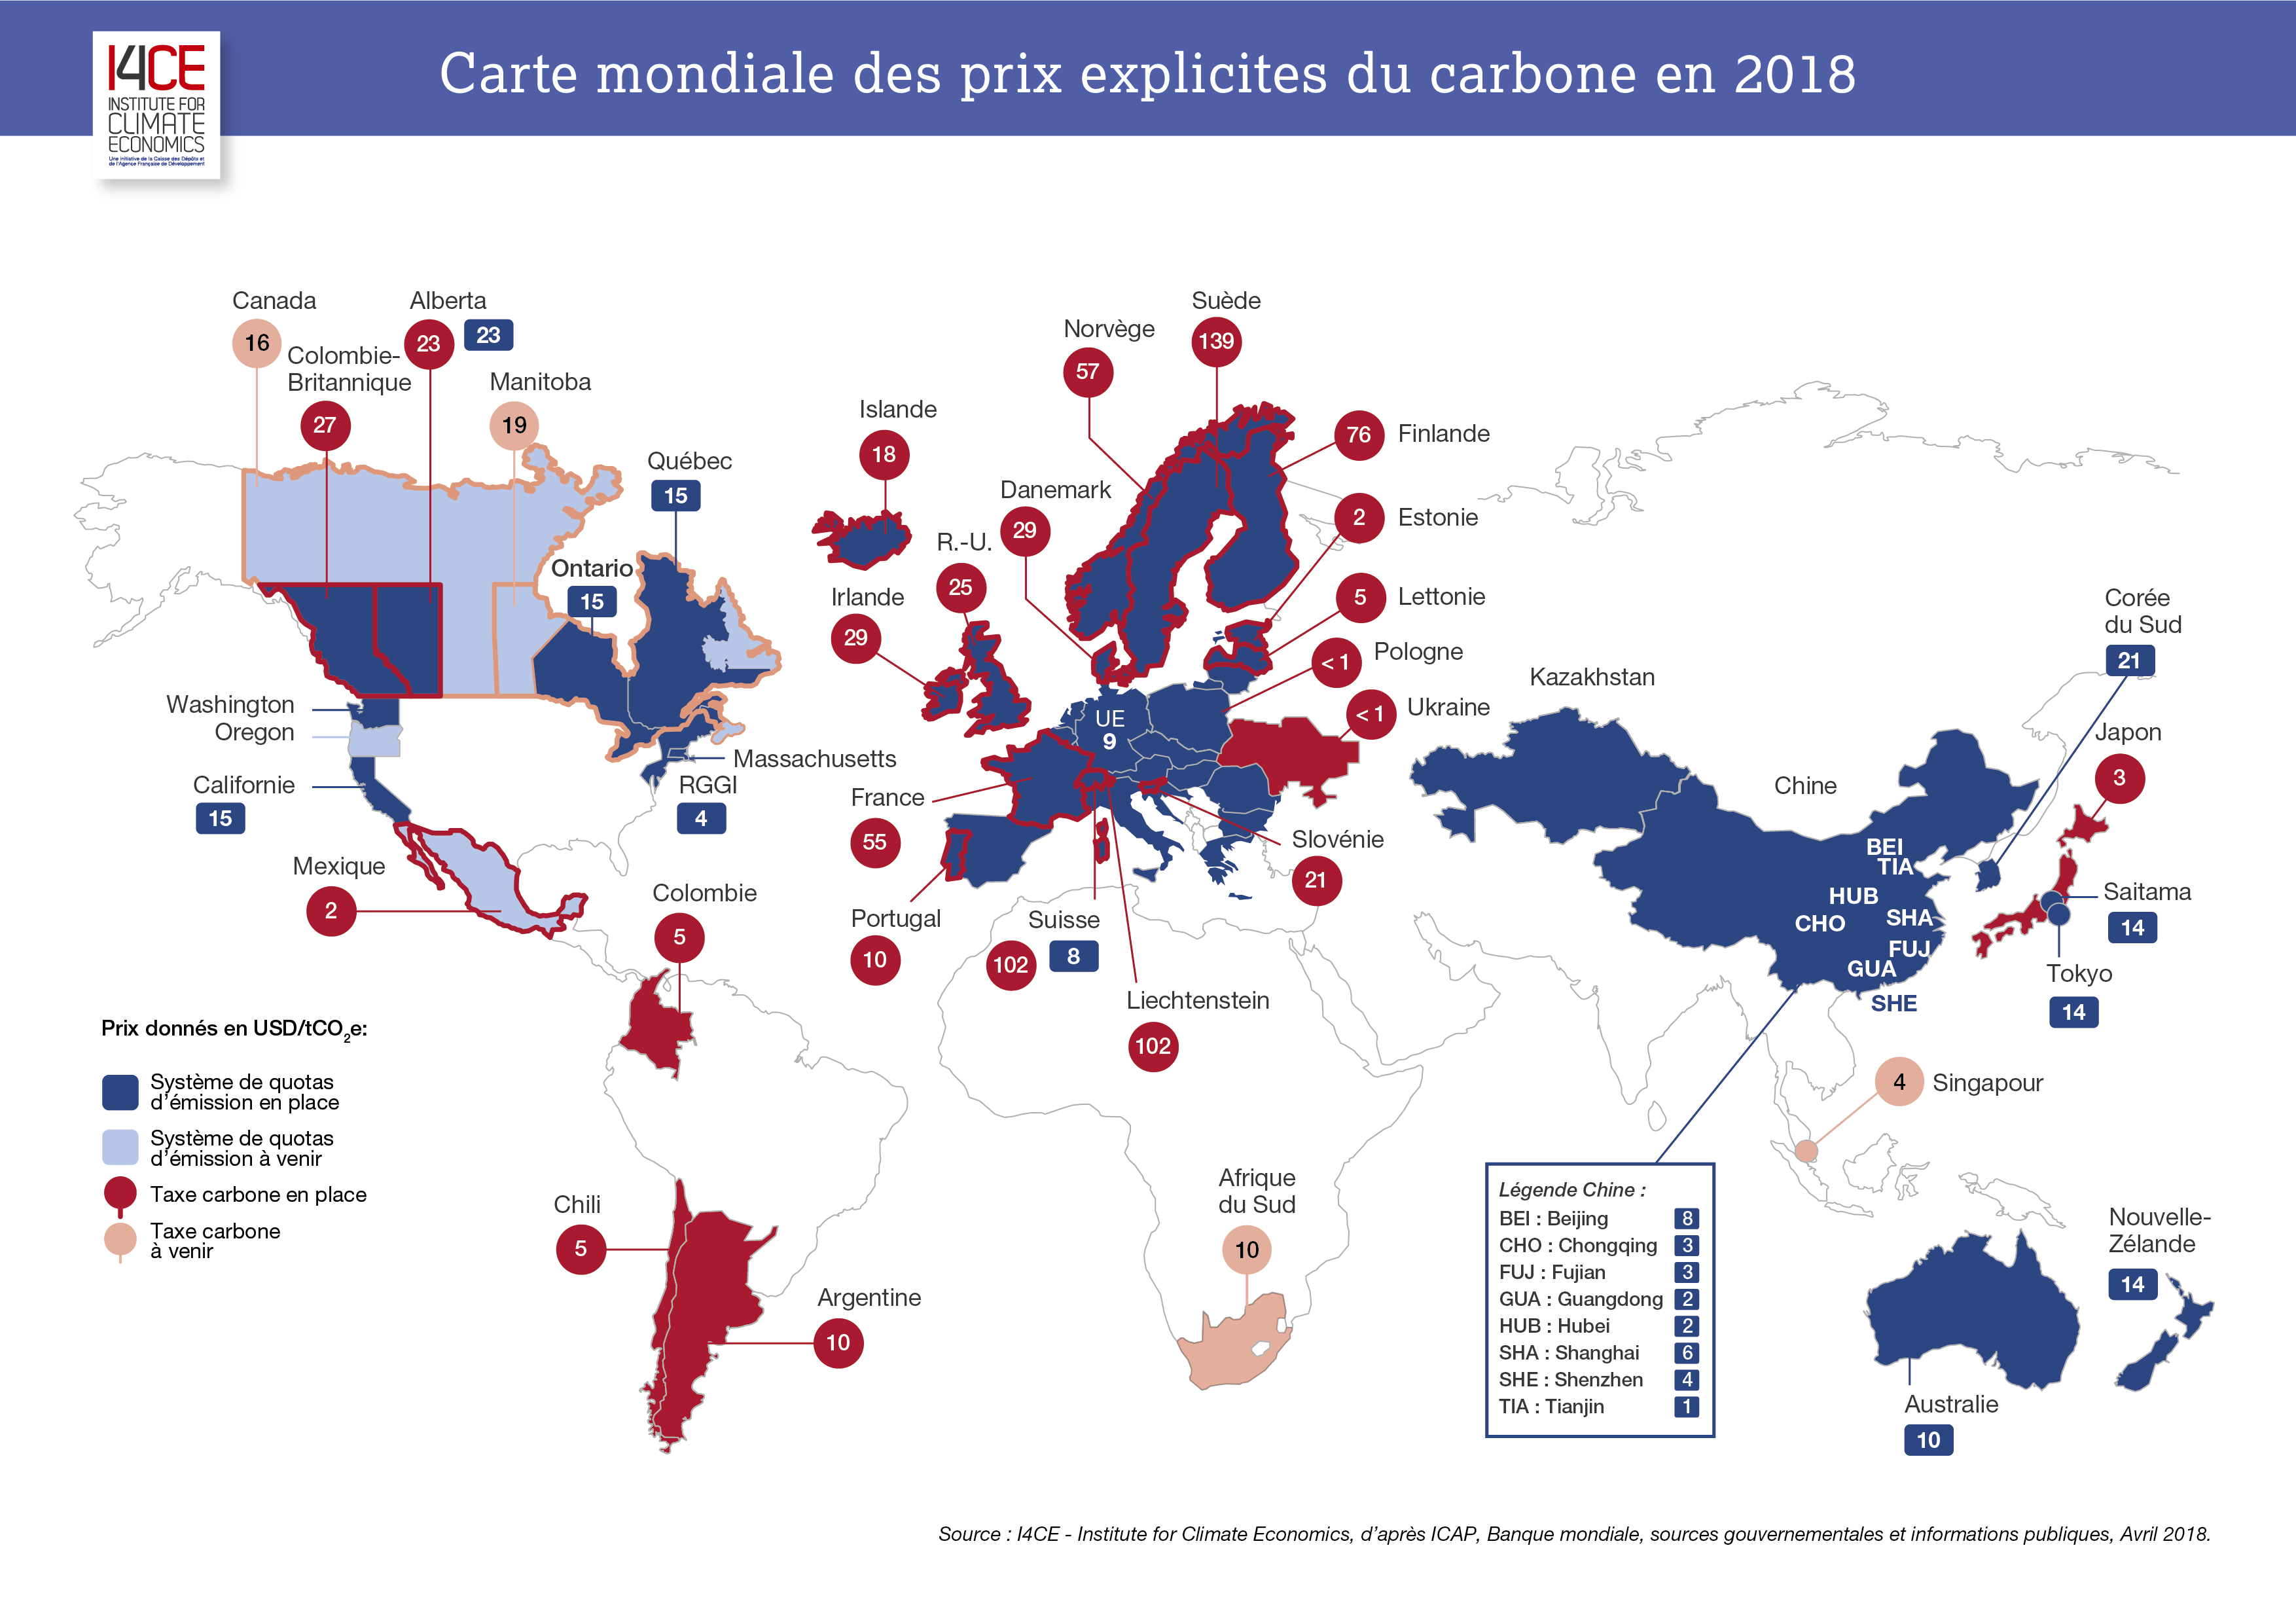
\includegraphics[width=\textwidth]{Informe/Carte-prix-du-carbone.png}
 
 \caption{Map of explicit carbon prices around the world in 2018. Taken from I4CE Institute for Climate Economics (https://www.i4ce.org/download/global-carbon-account-2018/)}
 \label{map-carbon-price}
\end{figure}

\subsection{Suggested Model for Cap-and-Trade Policy}
Our first approach is to present a simple outline to model the cap-and-trade market. Similar to Paper I, we start from stochastic equilibrium models, described in Section \ref{paperI}. The difference in our case is that the producers will not only optimize its profit (minimizing the cost, as shown before), but also will have to make a decision about the number of ``pollution permits'' that will trade in the second stage (spot market scenario). The pollution permits are limited by a regulatory agent. Ruiz et al. (2014) listed the four types of possible decisions that the produces might choose:

\begin{itemize}
    \item[1.] The producer decides to emit fewer tons of C02 (or other polluters), and thus, can sell the excess of permits, which is a revenue in profit. 
    
    \item[2.] The producer decides to emit more than the permits it has been given, therefore, it will need to buy extra permits in the trading market. 
    
    \item[3.] Producer uses ``soft'' strategies to reduce emissions. These strategies might be: 1. shifting output from ``dirty'' to ``cleaner'' plants (this method is known as emission dispatch\footnote{The emission dispatch problem is to determine the optimal combination of power outputs for all generating units which  minimizes the total emission (see Rezaie et al., 2018 and references therein).}); 2. the producer might reduce its sales; 3. purchase energy from cleaner suppliers; 4. switch to cleaner fuels within its plants.

    \item[4.] Producer decides on a ``hard''  drastic strategy: it removes old, dirty plants and invest in cleaner, more sustainable plants.
\end{itemize}

In our model, these decisions are represented by continuous variables. The equilibrium is then determined by establishing the KKT conditions for all the agents in a complementarity model, with a market clearing constraint somewhat with the form 

\[ 0 \leq \textrm{Emissions cap} - \textrm{Producers emissions} \perp \textrm{Price of permits} \geq 0 \]

We plan to add a more detailed format can be given to our model. For instance, the maximum amount of permits in the market will be considered an endogenous random. This asses the problem of uncertainty, a key feature of the power market (de Maere et al. 2018), and allows the model to obtain the most suitable amount of permits, considering different scenarios, a valuable information for policy-makers. Also, we have considered carbon emission, but other polluters might be included, like Nitrogen oxides (NOx), Sulfur oxides (SOx) and methane (CH$_{4}$), among others. The inclusion of these polluters may lead to a multicommodity analysis.  

In the next section we describe our first approach to model the cap-and-trade problem.

\subsection{Mathematical Formulation of the Model}\label{model}

Similar to Paper I, we will formulate a two stage capacity expansion model but including the cap-and-trade paradigm in the equations.

Let us consider a market of $i$ producers, each of them minimizing the cost of operation and investment. We will assume perfect competition among the producers. 

\smallskip

At first stage, we consider the current operating plant and the cost of the operation $C_i$, and the quantity produce $Q_i$. The maximum quantity of production at current stage (initial) is $\bar{Q}$. Each producer is allow to emit a certain amount of carbon $A_i$. We consider an auctioneer as the agent selling the allowances and obtaining a revenue for them. The revenue recipients are generally consumers (households) or low-emission companies. The auctioneer will try to maximize this revenue. In addition, we will consider the existence of a permit trading market, where producers can purchase permits from other producers if they need to surpass the emission allowances, or sell the unused permits if their emissions are below allowances. The total emission of each producer is $\varepsilon_i$. At this stage, the producer decides the amount $x$ of capacity expansion at a cost $I$ for the uncertain future. Next, at second stage, the producer wants to operate in the most efficient way at the spot market. We will evaluate the cost in the second stage as an expectation value and we will assume that the probability is a physical probability, which may be obtained from real world data. We have considered two stages as a simplification of the problem, but the analysis could be extended to a multistage problem. The variable that accounts for the time periods is $\tau$ (see below).
\smallskip

\begin{figure}[ht!]
 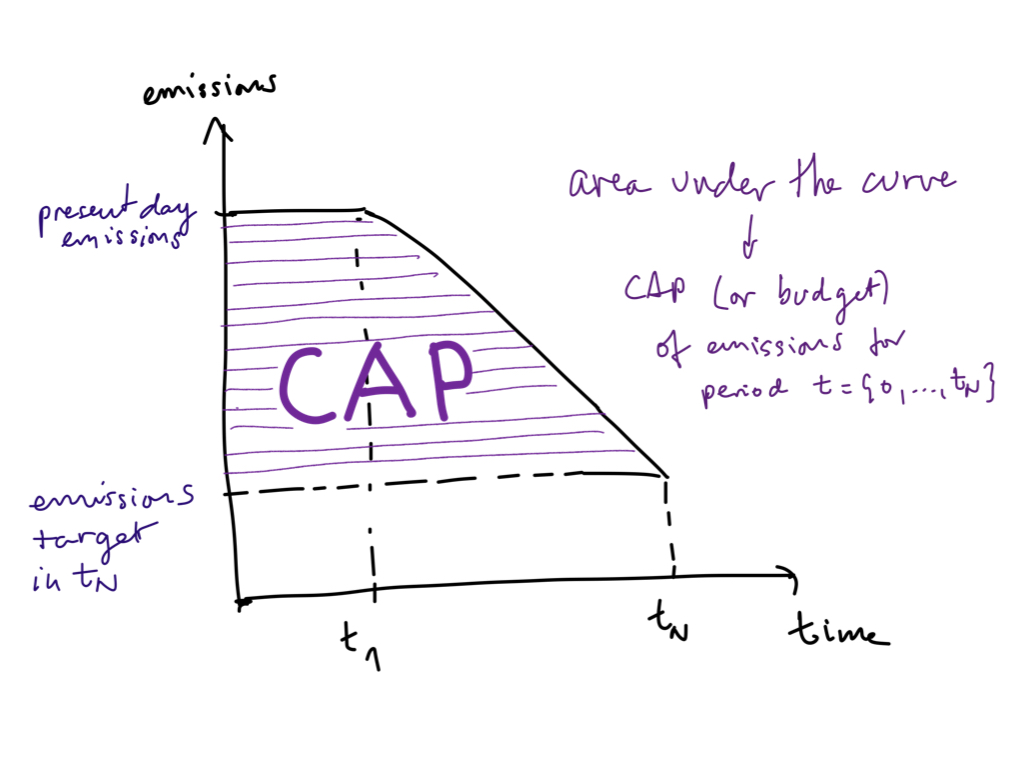
\includegraphics[width=\textwidth]{Informe/cap_scheme.jpeg}
 
 \caption{In a fix period of time, the total amount of carbon emissions allowed by a regulatory agent is CAP, that is, the area under the curve of the plot shown. The allowances sold to the different producers depend on each year, and the shape of the curve might vary, but the CAP, or maximum budget of emissions is fixed. }
 \label{cap-scheme}
\end{figure}

The maximum budget for emissions is the  parameter CAP, which in turn, follows a normal distribution, i.e., $CAP \thicksim N(\mu, \sigma^2)$. This CAP is determined by a regulatory agent and  accounts for the total emissions throughout the whole period considered, that is, does not depend of $\tau$. Figure \ref{cap-scheme} shows a simple scheme of CAP. In a period of years $\tau$, the emissions must be reduced in a certain amount to meet the target. For instance, Chile abides the Paris Agreement and is committed to reduce its emissions to 30\% below its 2007 levels by 2030\footnote{See https://climateactiontracker.org/countries/chile/ for a complete description of Chile's commitment in the Paris Agreement. Still, the promises made are categorized as highly insufficient to hold global warming below 2$^o$. }.

\smallskip
The amount of total allowances provided by the auctioneer $\theta$ is an endogenous random variable in our model, and it must satisfied the condition $\sum_i A_i = \theta$. 
Since $\theta$ must not surpass the budget for emissions, we consider a low margin (or risk) $R$ for this to happen, i.e.,
\begin{equation}
    P (\theta \geq CAP) \leq R
\end{equation}

and since the variable CAP follows a normal distribution with mean $\mu$ and variance $\sigma^2$, we can write the equation above as
\begin{equation}
    \theta \leq \phi^{-1}(R) \sigma^2 + \mu
\end{equation}

where $\phi^{-1}$ is the inverse of the cumulative function of the normal distribution. 



\hspace{0.5cm}

\begin{flushleft}
\textbf{Sets}
\begin{itemize}
    \item[] $i$: number of producers
    \item[] $\omega$: possible scenarios
    \item[] $\tau$: model periods
    
\end{itemize}

\hspace{0.5cm}

\textbf{Parameters}
\begin{itemize}
   \item[] $\bar{Q}_i$: maximum operation capacity
   \item[] $I$: expansion cost
   \item[] $C_i$: operation cost
   \item[] $D$: total demand (exogenous)
   \item[] $CAP$: maximum budget of emissions 
   \item[] $R$: margin for total emission allowances
\end{itemize}
\hspace{0.5cm}

\textbf{Variables}
\begin{itemize}
    \item[] $Q^{\tau}_i$: produced quantity
    \item[] $A^{\tau}_i$: emission allowances
    \item[] $P^{\tau}_i$: purchased permits
    \item[] $V^{\tau}_i$: sold permits
    \item[] $\lambda^{\tau}_i$: dual to CAP constraint
    \item[] $\mu^{\tau}_i$: dual to trading equilibrium
    \item[] $x_i$: capacity expansion decision
    \item[] $\theta_{\omega}$: emission permits available in the market
    \item[] $\varepsilon^{\tau}_{i,\omega}$: total emissions of producer $i$
    \end{itemize}

\hspace{0.5cm}

\textbf{Equations}\\

Each producer $i$ minimizes cost:
\begin{align}
    \min_{ x,Q,A,P,V} & \sum_{j}C_{i,j} Q^{1}_{i,j} + A^{1}_i\lambda^{1}_i + \sum_{j}I_{i,j}x_{i,j} \nonumber \\
     &\qquad - \sum_{\tau > 1} \sum_{\Omega}prob_\omega[\sum_j C_{i,j} Q^{\tau}_{i,j,\omega}  - (V^{\tau}_{i,\omega}-P^{\tau}_{i,\omega})\mu^{\tau}_{i,\omega}]\\
 \textrm{s.t \ } \nonumber
 \end{align}
 \begin{align}
 & Q^{\tau}_{i,j,\omega} \leq \bar{Q}_{i,j} + x_{i,j}  & \forall \ \omega, i, j, \tau \\
 & A^{\tau}_{i,\omega} + P^{\tau}_{i,\omega} \geq V^{\tau}_{i,\omega} & \forall \ \omega, i,\tau \\
 & Q^{\tau}_{i, j, \omega}\varepsilon^{\tau}_{i,\omega} \leq A^{\tau}_{i,\omega} + P^{\tau}_{i,\omega} - V^{\tau}_{i,\omega}  & \forall \ \omega, i,\tau \\
 & P^{\tau}_{i,\omega} \leq F(\sum_{\forall j \in J \subset K} x_{i,j}) & \forall i, j, \omega, \tau  \\
 & Q^{\tau}_{i, j, \omega} \geq 0  & \forall \ \omega, i, j, \tau
\end{align}

Auctioneer:
\begin{align}
    \max_{\theta} & \ \theta \lambda \\
    \textrm{s.t \ } & P(\theta \geq CAP) \leq R\\
    & \theta \geq 0
\end{align}

\textbf{Market clearing constraints}

\begin{align}
\textrm{(available allowances)}: &  \ \   \sum_{\tau} \sum_{i} A^{\tau}_{i,\omega} = \theta   & \forall \ \omega & \ \  (\lambda)\\
\textrm{(equilibrium in trading market)}: &   \ \  \sum_{i} P^{\tau}_{i,\omega} = \sum_{i} V^{\tau}_{i,\omega} & \forall \ \omega, \tau & \ \ (\mu) \\
\textrm{(fulfillment of the demand)}:  &   \ \  \sum_{i,j} Q^{\tau}_{i, j,\omega} = D^{\tau}_{\omega}, & \forall \ \omega, \tau & \ \ (\delta)
\end{align}

\end{flushleft}

The solution of this equilibrium problem will be estimated with a MCP formulation, as described in Section \ref{MCP}. 
\smallskip

Our model will also consider the case of incomplete markets. Again, the lack of information is an form of incompleteness, as discussed in Section \ref{paperI}. One way to include market incompleteness in our model is to consider some structure for the $V_i$ and $P_i$ variables, as a function of $x$ or some other variable. This motivates a discussion whether a solution exists, or in which cases is feasible. The details of this feature of our project are still under development. 

\section{Final Remarks}
We have discussed from first principles the topic of equilibrium problems, particularly in Energy markets. The model presented in Section \ref{model} is our first approach to tackle the problem. The next steps are to formulate the KKT conditions, at least for a ``toy model'' with some toy parameters. This will allow us to gain some insight about the model and to explore the limits of our assumptions. Then we will add real data from the chilean energy market. The idea is to compare the current carbon policy with the outcome of our model to evaluate its efficiency and provide policy-makers with other options for the market. Finally, we plan to study the feasibility of adding more complexities to the model, such a multiple power generation technologies and energy transmission, and solve them if possible.  

\begin{appendices}



\section{Example 3.3.1 from paper de Maere et. al. 2018 (working paper)}
In this example, there is one producer that can invest in one technology. 
The plant annual capital expenditure is $I= 90 \ \euro{} / kW$ and an operating cost of $60 \ \euro{} / MWh$.
The year is represented in a single segment of $\tau=8760$ hours. The producer is risk neutral.

The equation to minimize the producer cost of operation and initial investment is 
\[ \min_{x,Y}  Ix + \tau \mathbb{E}_{\Theta} [(C-P_{\omega}) Y_{\omega}]  \textrm{\  subject to \ }  0 \leq Y_{\omega} \leq x \]

The consumer is a price-taker agent with  a quadratic utility function $U_\omega(Q_\omega) = A_\omega Q_\omega - \frac{B}{2} Q_\omega^2$ and solves
\[ \min_{Q} \tau \mathbb{E}_\Theta \left[P_\omega Q_\omega - A_\omega Q_\omega + \frac{B}{2} Q_\omega^2 \right]\]

The quadratic term B is constant across the scenarios, with $B=1 \euro{}/MWh^2$.
The linear term $A_\omega$ is the only random parameter in the example. There are 5 scenarios ($K=5 \ , \ \mathcal{Z}=\mathbb{R}^5$), and an equal physical probability of $\Theta_\omega = 0.2$ for all $\omega$. The value of A is 

\begin{center}
\begin{tabular}{ c | c c c c c }
 $\omega$             & scen1 & scen2 & scen3 & scen4 & scen5 \\ 
 \hline
  $A \ [ \euro{}/MWh ] $ & 300   & 350   & 400   & 450   & 500 \\  
\end{tabular}
\end{center}



\subsection{Mixed complementarity problem}

\subsection{The producer}
The Lagrangian function for the producer problem is ($\lambda_1$ and $\lambda_2$ are Lagrange multipliers)

\[ \mathcal{L}= Ix + \tau \mathbb{E}_\Theta [(C-P_\omega) Y_\omega ] + \sum_w \lambda_{1,w} (Y_\omega -x) + \sum_w \lambda_{2,\omega}(0-Y_\omega) \]

The Karush-Kuhn-Tucker conditions  are:

\[ \frac{\partial \mathcal{L}}{\partial x}= I- \sum_{\omega}\lambda_{1,w} = 0  \]

\[\frac{\partial \mathcal{L}}{\partial Y_{\omega}} = \tau \Theta_\omega ( C - P_\omega ) + \lambda_{1, \omega} - \lambda_{2,\omega} =  0,\quad\omega\in\Omega \]

\vspace{1cm}

Primal feasibility :
\[ Y_\omega - x \leq 0 \quad  \forall \omega  \]
\[ 0 \leq Y_\omega \quad \forall \omega \]

Complementarity slackness: 

\[ (Y_\omega - x) \cdot \lambda_{1,\omega} = 0 \]
\[ Y_\omega \cdot \lambda_{2,\omega} = 0\]

Dual feasibility

\[ \lambda_{1,\omega} \geq 0 \quad \forall \omega \]
\[ \lambda_{2,\omega} \geq 0 \quad \forall \omega \]

We can write the KKT conditions as MCP as follows

\[ 0 \leq I- \sum_{\omega}\lambda_{1,w} \perp x \geq 0 \] 

\[ 0 \leq \tau \Theta_\omega C - \tau \Theta_\omega P_\omega + \lambda_{1,\omega} - \lambda_{2,\omega} \perp Y_\omega \geq 0, \quad \forall \omega\]

\[ 0 \leq x - Y_\omega \perp \lambda_{1,\omega} \geq 0 , \quad \forall \omega \]
\[ 0 \leq Y_\omega \perp \lambda_{2,\omega} \geq 0, \quad \forall \omega \]

\subsection{The consumer}

The KKT conditions for the consumer are as follows:

\[ 0 \leq \tau \Theta (P_\omega - A_\omega + B Q_\omega) \perp Q_\omega \geq 0\]




\subsection{Market clearing conditions}
 
 The market clearing constraint of the problem is 
\[ Y_\omega = Q_\omega \quad (P_\omega \  \textrm{dual})\]


\end{appendices}


\nocite{*}
\bibliographystyle{plain}
\bibliography{mybibliography}





\end{document}